%!TEX root = ../main.tex

\chapter{Distance estimation\label{chap:p3p}}

For distance estimation, one can leverage many different approaches, either directly relying on the event data stream itself, or integrating the
events over time (thus producing a grayscale image or a heatmap), and then estimating the position from the produced image. As we have shown in \refchap{chap:response}, the number of events
generated by LED sources decreases monotonically with the square of the distance and also decreases with increasing modulation frequency.
We could then assume that a simple distance predictor could be made by simply fitting a curve to the training dataset consisting of an average
number of events per blinking period (thus training this predictor for average number of events w. r. t. to distance) and then making the prediction of distance by calculating the average in real time.

This is possible to do in very specific cases where the camera settings and the scene lighting conditions do not change between training measurements
and the deployment. For example, changing the \texttt{bias-on} or \texttt{bias-off} settings of the camera changes the brightness change threshold on
which the camera generates events.
This changes the number of events that are generated without any information on the distance from the camera, this is similar to changing the eposure
time on a global shutter camera, which can then give an under- or over-exposed frame.
It also does not generalize the problem of estimating the position of an arbitrary UAV marked with LED lights and a camera with previously unspecified
settings. For a more robust way of estimating the pose of the UAV from the camera, we can leverage the following methods.

\section{RSSR}

The \ac{RSSR} method provides an approach to estimate the position of an object by measuring the relative ratio of received optical powers from \ac{LED}
markers. This is done by making each of the \ac{LED} markers radiate in their assigned time slot, measuring their optical powers at the time of the
radiation. Jung et al. (2014) \cite{sooyongrssr} demonstrated the \ac{RSSR} method using a configuration where four LED lamps were mounted on the ceiling
with a detector mounted on top of a moving object, parallel to the ceiling.
They have arrived at the equation \refeq{eq:rssr} which could be used to describe the power ratio $RSSR_{1,2}$
\begin{equation}
RSSR_{1,2} = \frac{P_{R1}}{P_{R2}} = \left( \frac{d_2}{d_1} \right)^{n+3}
\label{eq:rssr}
\end{equation}
where $P_{R1}$ and $P_{R2}$ are the received powers of the \ac{LED}s, $d_1$ and $d_2$ are the distances to the \ac{LED}s, and $n$ is the mode number of the radiation lobe (for a Lambertian model $n = 1$).

\section{Perspective-n-Point}
The \ac{PnP} problem addresses the estimation of the position of an object relative to the camera, having six degrees of freedom
\begin{itemize}
\item{Rotation - roll, pitch and yaw}
\item{Translation - 3D vector representing the position of the object relative to the camera}
\end{itemize}
This estimation is performed given a set of $n$ known 3D points $\{\mathbf{P}_i\}_{i=1}^n$ on the object and their corresponding 2D projections $\{\mathbf{p}_i\}_{i=1}^n$ in the image plane.
In our application, the UAV has four \ac{LED}-marked arms, where each of them can be distingushed by the camera as a point light source.
However, due to physical limits, only three \ac{LED}s will be visible at a single point in time, the fourth one behind obstructed by the physical structure of the \ac{UAV} when viewed from the front.
For a case of only 3 image points, the problem becomes the minimal solvable case, called \ac{P3P}, which 
can be formulated as a set of 3D points $\textbf{P}_i \in \mathbb{R}^{3}, i \in \{1, 2, 3\}$ in the world coordinate system, with their corresponding normalized image points
$\textbf{p}_i \in \mathbb{R}^{3}$, $|\textbf{p}_i|=1, i \in \{1, 2, 3\}$. These sets of points are related by a rigid transformation \cite{Ding_2023_CVPR}
\begin{equation}
d_i \textbf{p}_i = \textbf{R} \textbf{P}_i + \textbf{t}
\label{eq:p3p}
\end{equation}
where $d_i \in \mathbb{R}^+$.
Given the rigid transformation relationship shown in \refeq{eq:p3p}, the \ac{P3P} problem reduces to solving for the rotation matrix 
$\mathbf{R} \in \text{SO}(3)$, translation vector $\mathbf{t} \in \mathbb{R}^3$, and depths $d_i > 0$. 
By exploiting geometric constraints between the 3D points and their 2D projections, the problem can be
reformulated algebraically and solved using various techniques. In our approach, we use the method proposed by Kneip et al. \cite{kneip}, which
directly finds the rotation and translation with a novel parameterization of the model.
The visualization of the \ac{P3P} problem is shown on \reffig{fig:p3p}.
\begin{figure}[H]
	\centering
	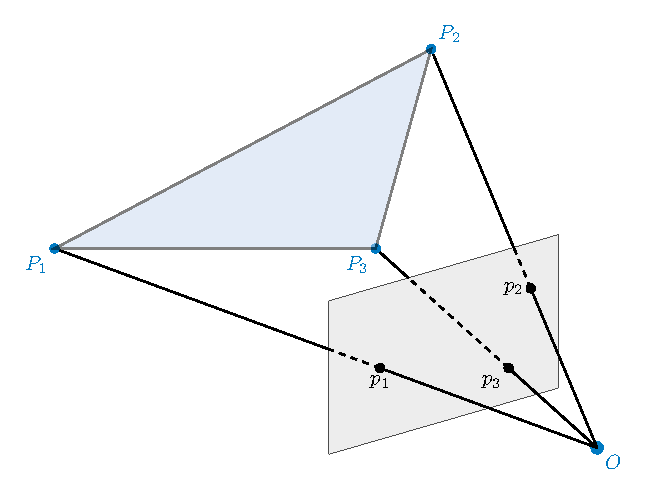
\includegraphics[width=0.65\textwidth]{./fig/tikz/p3p.pdf}
	\caption{P3P problem visualization}
	\label{fig:p3p}
\end{figure}
In our implementation, we compute the average of the estimated pose and distance, thus simplifying the problem of identifying the correct solution. If all four \ac{LED}s on the \ac{UAV} are detected, a general \ac{PnP} solution is calculated using the \ac{RANSAC} method. This yields only one solution, so the
estimated distance is simply the distance from the camera to the geometrical center of the \ac{UAV}.

\section{ROS implementation}
For the ease of deployement on real hardware, a distance estimator ROS node was implemented. The functionality can be summarized with the flowchart on
\reffig{fig:rosflow}.

\begin{figure}[H]
	\centering
	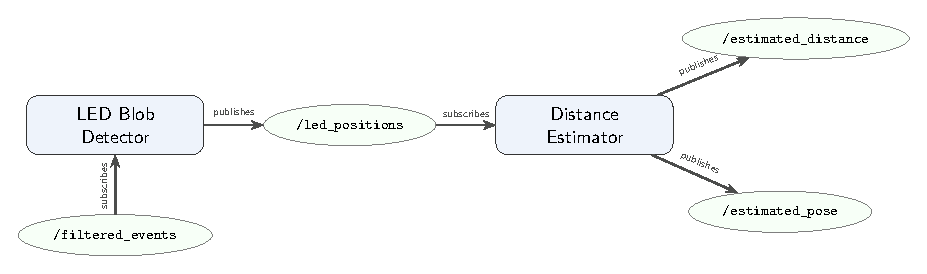
\includegraphics[width=1.0\textwidth]{./fig/tikz/rosflow.pdf}
	\caption{ROS distance estimation pipeline}
	\label{fig:rosflow}
\end{figure}


